% ====================================================================
%+
% SECTION NAME:
%    lenstimedelays.tex
%
% CHAPTER:
%    cosmology.tex
%
% ELEVATOR PITCH:
%    Lensed quasars and supernovae provide distance measurements for
%    cosmology. They are a few days to a few weeks in length. To
%    measure them well we need long campaigns (>~3 years) with high
%    night-to-night cadence (better than the standard 5 days if
%    possible, especially as combining all filters might be difficult.)
%
% AUTHORS:
%   Phil Marshall (@drphilmarshall)
%-
% ====================================================================

\section{ Strong Gravitational Lens Time Delays }
\def\secname{lenstimedelays}\label{sec:\secname}

\credit{drphilmarshall},
\credit{rhiannonlynne},
\credit{tanguita}

The multiple images of strongly lensed quasars and supernovae have
delayed arrival times: variability in the first image will be observed
in the second image some time later, as the photons take different
paths around the deflector galaxy, and through different depths of
gravitational potential. If the lens mass distribution can be modeled
independently, using a combination of high resolution imaging of the
distorted quasar/SN host galaxy and stellar dynamics in the lens
galaxy, the measured time delays can be used to infer the ``time delay
distance'' in the system. This distance enables a direct measurement
of the Hubble constant, independent of the distance ladder.

% --------------------------------------------------------------------

\subsection{Target measurements and discoveries}
\label{sec:\secname:targets}

For this cosmological probe to be competitive with LSST's others, the
time delays of several hundred systems (which will be distributed
uniformly over the extragalactic sky) will need to be measured with
bias below the sub-percent level, while the precision required is a
few percent per lens.  In galaxy-scale lenses, the kind that are most
accurately modeled, these time delays are typically between several
days and several weeks long, and so are measurable in monitoring
campaigns having night-to-night cadence of between one and a few days,
and seasons lasting several months or more.

To obtain accurate as well as precise lensed quasar time delays, several
monitoring seasons are required. Lensed supernova time delays have not
yet been measured, but their transient nature means that their time
delay measurements may be more sensitive to cadence than season or
campaign length.

% --------------------------------------------------------------------

\subsection{Metrics}
\label{sec:\secname:metrics}

Anticipating that the time delay accuracy would depend on night-to-night
cadence, season length, and campaign length, we carried out a large
scale simulation and measurement program that coarsely sampled these
schedule properties. In \citet{LiaoEtal2015}, we simulated 5 different
light curve datasets, each containing 1000 lenses, and presented them to
the strong lensing community in a ``Time Delay Challenge.'' These 5
challenge ``rungs'' differed by their schedule properties, in the ways
shown in \autoref{tab:tdcrungs}. Focusing on the best challenge
submissions made by the community, we derived a simple power law model
for the variation of each of the time delay accuracy, time delay
precision, and useable sample fraction, with the schedule properties
cadence, season length and campaign length. These models are shown in
\autoref{fig:tdcresults}, reproduced from \citet{LiaoEtal2015}, and are
given by the following equations:
\begin{align}
|A|_{\rm model} &\approx 0.06\% \left(\frac{\rm cad} {\rm 3 days}  \right)^{0.0}
                          \left(\frac{\rm sea}  {\rm 4 months}\right)^{-1.0}
                          \left(\frac{\rm camp}{\rm 5 years} \right)^{-1.1} \notag \\
  P_{\rm model} &\approx 4.0\% \left(\frac{\rm cad} {\rm 3 days}  \right)^{ 0.7}
                         \left(\frac{\rm sea}  {\rm 4 months}\right)^{-0.3}
                         \left(\frac{\rm camp}{\rm 5 years} \right)^{-0.6} \notag \\
  f_{\rm model} &\approx 30\% \left(\frac{\rm cad} {\rm 3 days}  \right)^{-0.4}
                        \left(\frac{\rm sea}  {\rm 4 months}\right)^{ 0.8}
                        \left(\frac{\rm camp}{\rm 5 years} \right)^{-0.2} \notag
\end{align}

%%%%%%%%%%%%%%%%%%%%%%%%%%%%%%%%%%%%
\begin{table*}
\begin{center}
\capstart
\begin{tabular}{cccccc} \hline\hline
  Rung &  Mean Cadence & Cadence Dispersion & Season   & Campaign & Length   \\
       &  (days)       & (days)             & (months) & (years)  & (epochs) \\ \hline
  0    &    3.0        &   1.0              &   8.0    &    5     & 400      \\
  1    &    3.0        &   1.0              &   4.0    &    10    & 400      \\
  2    &    3.0        &   0.0              &   4.0    &    5     & 200      \\
  3    &    3.0        &   1.0              &   4.0    &    5     & 200      \\
  4    &    6.0        &   1.0              &   4.0    &    10    & 200      \\
\hline\hline
\end{tabular}
\end{center}
\caption{The observing parameters for the five rungs of the Time Delay
Challenge. Reproduced from \citet{LiaoEtal2015}.\label{tab:tdcrungs}}
\end{table*}
%%%%%%%%%%%%%%%%%%%%%%%%%%%%%%%%%%%%

%%%%%%%%%%%%%%%%%%%%%%%%%%%%%%%%%%%
\begin{figure*}[!ht]
  \capstart
  \begin{minipage}[b]{\linewidth}
    \begin{minipage}[b]{0.32\linewidth}
      \centering\includegraphics[width=\linewidth]{figs/Accuracy_season_nca.pdf}
    \end{minipage} \hfill
    \begin{minipage}[b]{0.32\linewidth}
      \centering\includegraphics[width=\linewidth]{figs/Precision_cadence_nca.pdf}
    \end{minipage} \hfill
    \begin{minipage}[b]{0.32\linewidth}
      \centering\includegraphics[width=\linewidth]{figs/Fraction_season_nca.pdf}
    \end{minipage}
  \end{minipage}
\caption{Examples of changes in accuracy $A$ (left), precision $P$
(center) and success fraction $f$ (right) with schedule properties, as
seen in the different TDC submissions. The gray approximate power law
model was derived by visual inspection of the pyCS-SPL results; the
signs of the indices were pre-determined according to our expectations.
Reproduced from \citet{LiaoEtal2015}.}
\label{fig:tdcresults}
\end{figure*}
%%%%%%%%%%%%%%%%%%%%%%%%%%%%%%%%%%%

All three of these diagnostic metrics would, in an ideal world, be
optimized: this could be achieved by decreasing the night-to-night
cadence (to better sample the light curves), extending the observing
season length (to maximize the chances of capturing a strong variation
and its echo), and extending the campaign length (to increase the number
of effective time delay measurements).

The quantity of greatest scientific interest is the {\it accuracy in
cosmological parameters}: this could be computed as follows. Setting a
required accuracy threshold  defines the available number of lenses,
which in turns gives us the mean precision per lens there. Combining the
whole sample, we would get the error on the weighted mean time delay, as
used by \citet{Coe+Moustakas2009}. This uncertainty, which scales as one
over the square root of the number of available lenses,  can be roughly
equated to the statistical uncertainty on the Hubble constant. The
Figure of Merit would be the final percentage precision on $H_0$, as a
way to sum up the sample size and time delay measurability (at fixed
accuracy requirement).

% --------------------------------------------------------------------

\subsection{\OpSim Analysis}
\label{sec:\secname:analysis}

% \OpSim analysis: how good would the default observing strategy be, at
% the time of writing for this science project?

In this section we present the results of our ongoing \OpSim / MAF
analysis, as we start to try to
answer the question ``how good would the proposed observing
strategies be, for time delay lens cosmography?''

\autoref{fig:lenstimedelays:accuracymaps} shows maps of TDC2 time delay
measurement accuracy from our MAF analysis of two \OpSim databases, the
baseline cadence \opsimdbref{db:baseCadence}, and a ``No Visit Pairs''
strategy, \opsimdbref{db:NoVisitPairs}. We use the \metric{TdcMetric} to compare three different
analysis scenarios, differing by a) whether or not we can combine all 6
filters' light curves such that they behave like the TDC2 single-filter
simulations (as was assumed by \citeauthor{LiaoEtal2015}), and b)
whether we wait 5 or 10 years before making the time delay measurement.\footnote{Here, ``years'' means ``seasons:'' we used the
\metric{SeasonStacker} to work
with seasons, rather than calendar years.}

These sky maps saturate at a threshold of 0.04\%, chosen conservatively
to be 5 times stricter than that used by
\citeauthor{Hojjati+Linder2014}. We can see that the area of sky
providing lenses measurable at this accuracy or better increases
markedly as we move from $ri$ to $ugrizy$. These maps predict that while
the accuracy should increase between DR5 and DR10, the sky area yielding
accuracy better than 0.04\% should already be close to the full WFD area
(18000 square degrees) by DR5: this bodes well for our ability to make
use of shorter campaign sky areas observed at higher frequency, as would
emerge from a rolling cadence strategy.

To summarize the diagnostic metric results, we first compute the area of
this ``high accuracy'' sky. We can then compute the cadence, season, and
campaign length just in these areas; these values are reported in
\autoref{tab:lenstimedelays:results}. The high accuracy area can be used
to define a ``Gold Sample'' of lenses, whose mean precision per lens we
can compute. The TDC2 useable fraction averaged over this area gives us
the approximate size of this sample: we simply re-scale the 400 lenses
predicted by \citet{LiaoEtal2015} by this fraction over the 30\% found
in TDC2. While these numbers are approximate, the ratios between
different observing and analysis strategies provide a useful indication of relative merit.

As described above, we follow \citet{Coe+Moustakas2009} and compute a
very simple time delay distance Figure of Merit ``\texttt{DPrecision}''
as follows. We first combine the fractional time delay precision in
quadrature with an assumed 4\% ``modeling uncertainty,'' and then divide
this by the square root of the number of Gold Sample lenses. This
estimated ensemble distance precision can be straightforwardly related
to cosmological parameter precision, as \citet{Coe+Moustakas2009} show
(it's very roughly the precision on the Hubble constant).  This distance
precision Figure of Merit is given in the final column of
\autoref{tab:lenstimedelays:results}. We see that in DR5, being able to
combine all filters instead of just $ri$ should give a FoM of 0.29\%
instead of 1.25\%; between DR5 and DR10 this then should improve to
0.24. This suggests that time delay measurement is primarily {\it
analysis-limited}. In the ``No Visit Pairs'' strategy, we seet that the
DR5 all-band FoM is 0.26\%, just a 10\% improvement. This might be
because the ``No Visit Pairs'' does not {\it insist} that the visits in
the visit pairs are split over different nights, only that they don't
{\it have} to be taken on the same night. We might expect a more
aggressive approach to splitting visit pairs to make a bigger difference --
but it seems unlikely that it would be a factor of two improvement.

%%%%%%%%%%%%%%%%%%%%%%%%%%%%%%%%%%%
\begin{figure*}[!ht]
  \capstart
  \begin{minipage}[b]{\linewidth}
    \begin{minipage}[b]{0.48\linewidth}
       \centering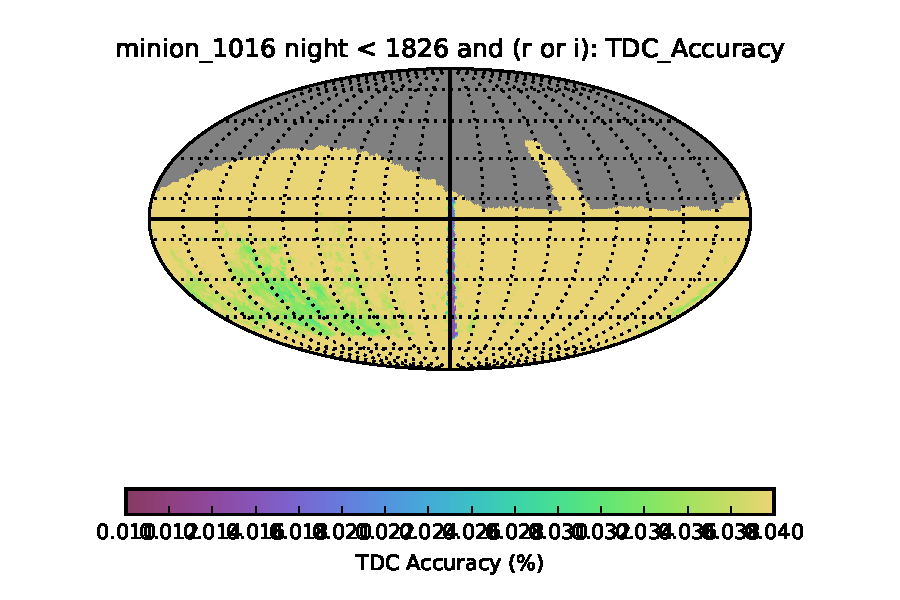
\includegraphics[width=\linewidth]{figs/lenstimedelays/minion_1016_TDC_Accuracy_night_lt_1826_and_r_or_i_HEAL_SkyMap.pdf}
    \end{minipage} \hfill
    \begin{minipage}[b]{0.48\linewidth}
       \centering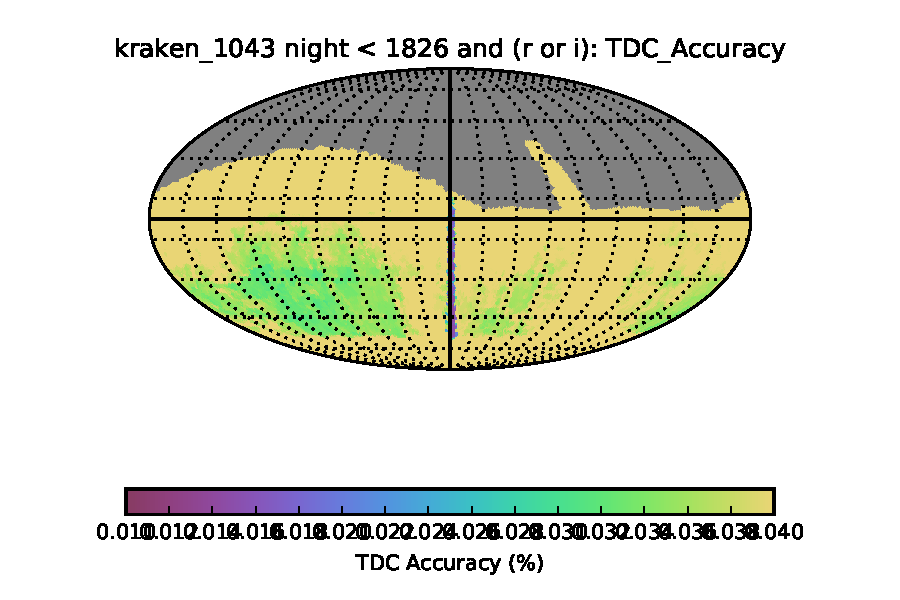
\includegraphics[width=\linewidth]{figs/lenstimedelays/kraken_1043_TDC_Accuracy_night_lt_1826_and_r_or_i_HEAL_SkyMap.pdf}
    \end{minipage}
  \end{minipage}
  \begin{minipage}[b]{\linewidth}
    \begin{minipage}[b]{0.48\linewidth}
       \centering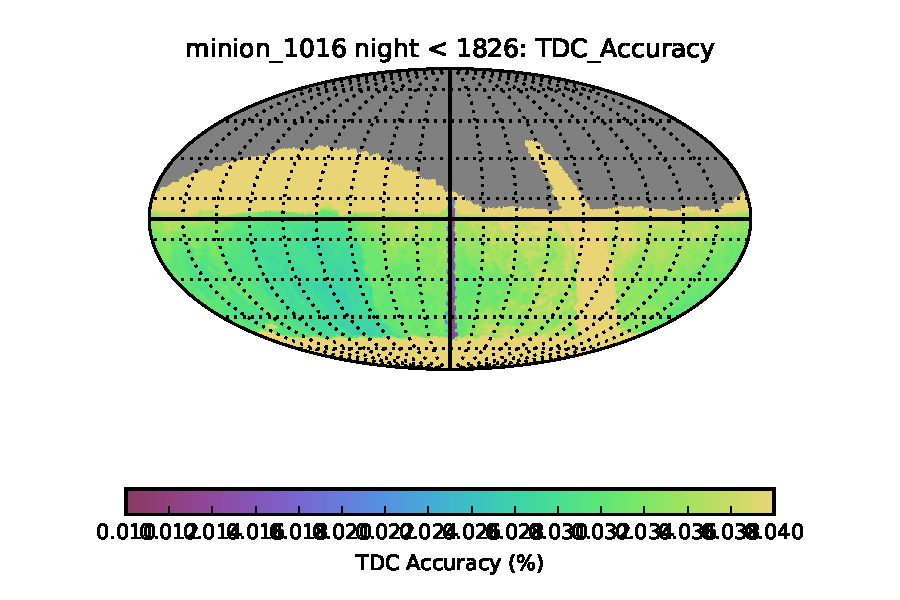
\includegraphics[width=\linewidth]{figs/lenstimedelays/minion_1016_TDC_Accuracy_night_lt_1826_HEAL_SkyMap.pdf}
    \end{minipage} \hfill
    \begin{minipage}[b]{0.48\linewidth}
       \centering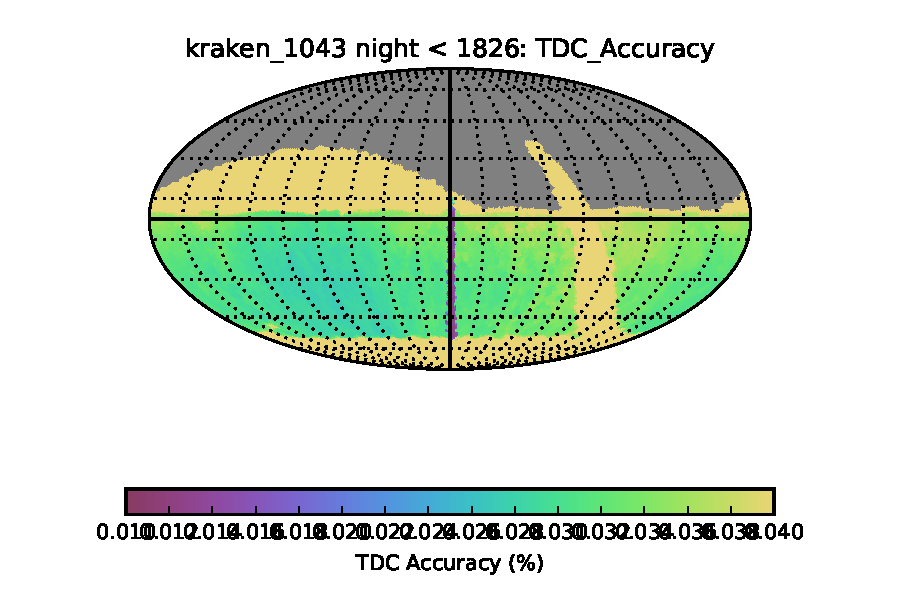
\includegraphics[width=\linewidth]{figs/lenstimedelays/kraken_1043_TDC_Accuracy_night_lt_1826_HEAL_SkyMap.pdf}
    \end{minipage}
  \end{minipage}
  \begin{minipage}[b]{\linewidth}
    \begin{minipage}[b]{0.48\linewidth}
       \centering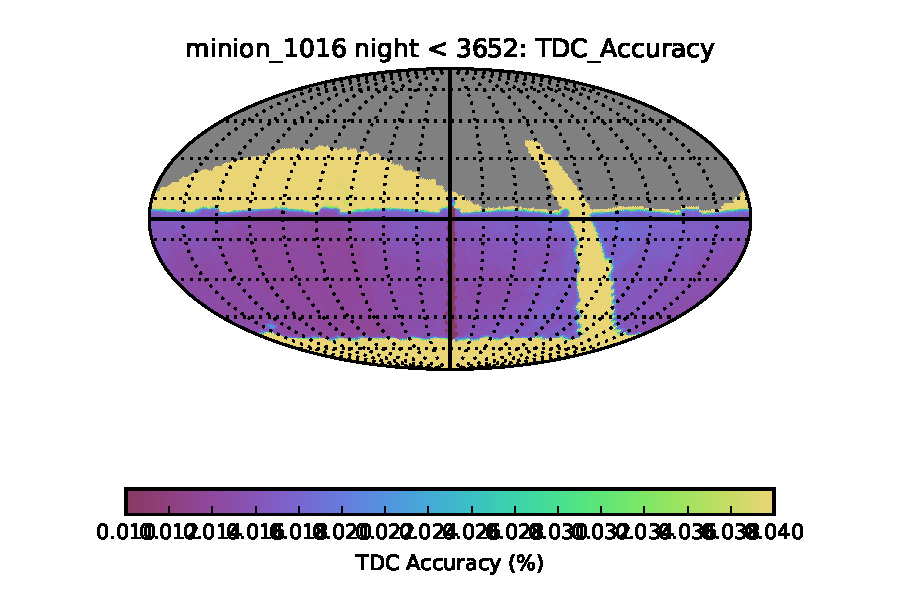
\includegraphics[width=\linewidth]{figs/lenstimedelays/minion_1016_TDC_Accuracy_night_lt_3652_HEAL_SkyMap.pdf}
    \end{minipage} \hfill
    \begin{minipage}[b]{0.48\linewidth}
       \centering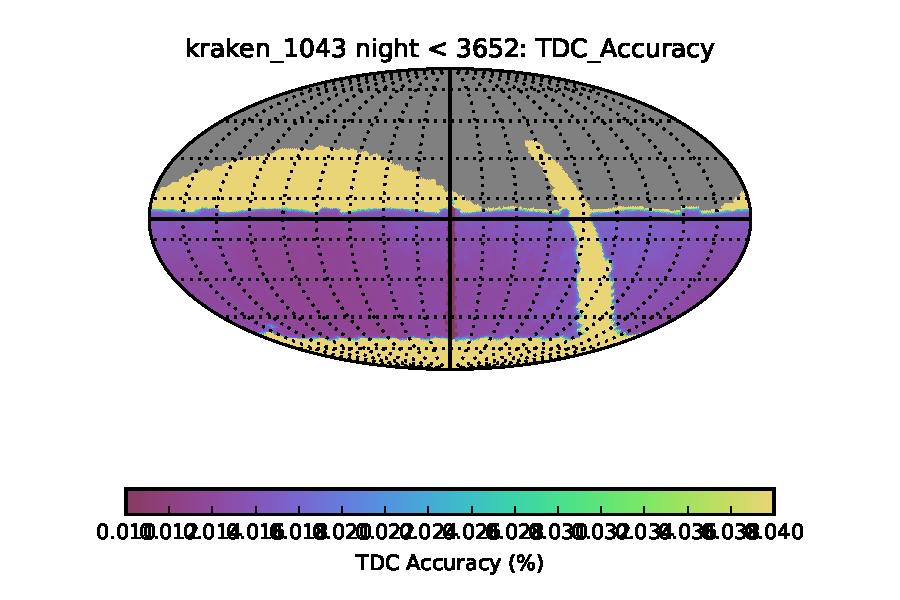
\includegraphics[width=\linewidth]{figs/lenstimedelays/kraken_1043_TDC_Accuracy_night_lt_3652_HEAL_SkyMap.pdf}
    \end{minipage}
  \end{minipage}
\caption{Sky maps of the TDC2 time delay measurement accuracy metric $A$ for the baseline cadence \opsimdbref{db:baseCadence} (left) and the ``No Visit Pairs'' strategy, \opsimdbref{db:NoVisitPairs} (right). The rows show the build up of data quality with time and analysis capability, from 5 years of $r$ and $i$-band light curve data only (top row), to 5 years of hypothetically-combined $ugrizy$ light curve data (middle row), to 10 years of hypothetically-combined $ugrizy$ light curve data (bottom row). The maps saturate at the threshold accuracy of 0.04, such that any regions that are {\it not yellow} should yield high accuracy lens time delays.}
\label{fig:lenstimedelays:accuracymaps}
\end{figure*}
%%%%%%%%%%%%%%%%%%%%%%%%%%%%%%%%%%%

% List of possible skymaps, oh my:
%
% kraken_1043_TDC_Accuracy_night_lt_1826_HEAL_SkyMap.pdf
% kraken_1043_TDC_Accuracy_night_lt_1826_and_r_or_i_HEAL_SkyMap.pdf
% kraken_1043_TDC_Accuracy_night_lt_3652_HEAL_SkyMap.pdf
% kraken_1043_TDC_Accuracy_night_lt_3652_and_r_or_i_HEAL_SkyMap.pdf
% kraken_1043_TDC_Cadence_night_lt_1826_HEAL_SkyMap.pdf
% kraken_1043_TDC_Cadence_night_lt_1826_and_r_or_i_HEAL_SkyMap.pdf
% kraken_1043_TDC_Cadence_night_lt_3652_HEAL_SkyMap.pdf
% kraken_1043_TDC_Cadence_night_lt_3652_and_r_or_i_HEAL_SkyMap.pdf
% kraken_1043_TDC_Campaign_night_lt_1826_HEAL_SkyMap.pdf
% kraken_1043_TDC_Campaign_night_lt_1826_and_r_or_i_HEAL_SkyMap.pdf
% kraken_1043_TDC_Campaign_night_lt_3652_HEAL_SkyMap.pdf
% kraken_1043_TDC_Campaign_night_lt_3652_and_r_or_i_HEAL_SkyMap.pdf
% kraken_1043_TDC_Precision_night_lt_1826_HEAL_SkyMap.pdf
% kraken_1043_TDC_Precision_night_lt_1826_and_r_or_i_HEAL_SkyMap.pdf
% kraken_1043_TDC_Precision_night_lt_3652_HEAL_SkyMap.pdf
% kraken_1043_TDC_Precision_night_lt_3652_and_r_or_i_HEAL_SkyMap.pdf
% kraken_1043_TDC_Rate_night_lt_1826_HEAL_SkyMap.pdf
% kraken_1043_TDC_Rate_night_lt_1826_and_r_or_i_HEAL_SkyMap.pdf
% kraken_1043_TDC_Rate_night_lt_3652_HEAL_SkyMap.pdf
% kraken_1043_TDC_Rate_night_lt_3652_and_r_or_i_HEAL_SkyMap.pdf
% kraken_1043_TDC_Season_night_lt_1826_HEAL_SkyMap.pdf
% kraken_1043_TDC_Season_night_lt_1826_and_r_or_i_HEAL_SkyMap.pdf
% kraken_1043_TDC_Season_night_lt_3652_HEAL_SkyMap.pdf
% kraken_1043_TDC_Season_night_lt_3652_and_r_or_i_HEAL_SkyMap.pdf
% minion_1016_TDC_Accuracy_night_lt_1826_HEAL_SkyMap.pdf
% minion_1016_TDC_Accuracy_night_lt_1826_and_r_or_i_HEAL_SkyMap.pdf
% minion_1016_TDC_Accuracy_night_lt_3652_HEAL_SkyMap.pdf
% minion_1016_TDC_Accuracy_night_lt_3652_and_r_or_i_HEAL_SkyMap.pdf
% minion_1016_TDC_Cadence_night_lt_1826_HEAL_SkyMap.pdf
% minion_1016_TDC_Cadence_night_lt_1826_and_r_or_i_HEAL_SkyMap.pdf
% minion_1016_TDC_Cadence_night_lt_3652_HEAL_SkyMap.pdf
% minion_1016_TDC_Cadence_night_lt_3652_and_r_or_i_HEAL_SkyMap.pdf
% minion_1016_TDC_Campaign_night_lt_1826_HEAL_SkyMap.pdf
% minion_1016_TDC_Campaign_night_lt_1826_and_r_or_i_HEAL_SkyMap.pdf
% minion_1016_TDC_Campaign_night_lt_3652_HEAL_SkyMap.pdf
% minion_1016_TDC_Campaign_night_lt_3652_and_r_or_i_HEAL_SkyMap.pdf
% minion_1016_TDC_Precision_night_lt_1826_HEAL_SkyMap.pdf
% minion_1016_TDC_Precision_night_lt_1826_and_r_or_i_HEAL_SkyMap.pdf
% minion_1016_TDC_Precision_night_lt_3652_HEAL_SkyMap.pdf
% minion_1016_TDC_Precision_night_lt_3652_and_r_or_i_HEAL_SkyMap.pdf
% minion_1016_TDC_Rate_night_lt_1826_HEAL_SkyMap.pdf
% minion_1016_TDC_Rate_night_lt_1826_and_r_or_i_HEAL_SkyMap.pdf
% minion_1016_TDC_Rate_night_lt_3652_HEAL_SkyMap.pdf
% minion_1016_TDC_Rate_night_lt_3652_and_r_or_i_HEAL_SkyMap.pdf
% minion_1016_TDC_Season_night_lt_1826_HEAL_SkyMap.pdf
% minion_1016_TDC_Season_night_lt_1826_and_r_or_i_HEAL_SkyMap.pdf
% minion_1016_TDC_Season_night_lt_3652_HEAL_SkyMap.pdf
% minion_1016_TDC_Season_night_lt_3652_and_r_or_i_HEAL_SkyMap.pdf

%%%%%%%%%%%%%%%%%%%%%%%%%%%%%%%%%%%%%%

\begin{table*}
\begin{center}
\caption{Lens Time Delay Metric Analysis Results.}
\label{tab:lenstimedelays:results}
\footnotesize
\begin{tabularx}{\linewidth}{ccccccccc}
  \hline
  \OpSim run                       % runName -> db
   & Filters                       % filters
    & Years                        % Nyears
     & \texttt{cadence}            % high_accuracy_cadence
      & \texttt{season}            % high_accuracy_season
       & \texttt{Area}             % high_accuracy_area
        & \texttt{dtPrecision}     % precision_per_lens
         & \texttt{Nlenses}        % N_lenses
          & \texttt{DPrecision} \\ % distance_precision
  \hline\hline
  \opsimdbref{db:baseCadence}
   & $ugrizy$
    & $10$
     & $4.5$
      & $6.9$
       & $19004$
        & $5.09$
         & $468$
          & $0.24$ \\
  \opsimdbref{db:baseCadence}
   & $ugrizy$
    & $5$
     & $5.1$
      & $6.6$
       & $17926$
        & $6.29$
         & $472$
          & $0.29$ \\
  \opsimdbref{db:baseCadence}
   & $ri$
    & $10$
     & $10.4$
      & $5.7$
       & $18566$
        & $7.07$
         & $285$
          & $0.42$ \\
  \opsimdbref{db:baseCadence}
   & $ri$
    & $5$
     & $14.2$
      & $5.5$
       & $4841$
        & $10.81$
         & $75$
          & $1.25$ \\
  \opsimdbref{db:NoVisitPairs}
   & $ugrizy$
    & $10$
     & $3.9$
      & $7.1$
       & $18907$
        & $4.88$
         & $502$
          & $0.22$ \\
  \opsimdbref{db:NoVisitPairs}
   & $ugrizy$
    & $5$
     & $4.5$
      & $6.7$
       & $18093$
        & $5.93$
         & $504$
          & $0.26$ \\
  \opsimdbref{db:NoVisitPairs}
   & $ri$
    & $10$
     & $8.5$
      & $6.1$
       & $18617$
        & $6.34$
         & $329$
          & $0.35$ \\
  \opsimdbref{db:NoVisitPairs}
   & $ri$
    & $5$
     & $10.7$
      & $6.1$
       & $9358$
        & $9.35$
         & $171$
          & $0.71$ \\
   \hline

\multicolumn{9}{p{\linewidth}}{\scriptsize Notes: see the text for
the definitions of each metric.}
\end{tabularx}
\normalsize
\medskip\\
\end{center}
\end{table*}
%%%%%%%%%%%%%%%%%%%%%%%%%%%%%%%%%%%%%%


% --------------------------------------------------------------------

\subsection{Discussion}
\label{sec:\secname:discussion}

The main risk involved with this science case is that the
``multi-filter'' light curve analysis presented here, which extrapolates
from the results of the single-filter TDC1, does not represent
accurately the real-life combination of all 6 filters together. The
second time delay challenge (TDC2) will help answer this question.  For
now, just using 2 filters gives an upper limit on the overall precision
we should expect.

Naively, we would expect the relaxation of the visit pairs requirement
to increase the  night-to-night cadence by a factor of two, if the
visits are redistributed randomly in time. However, it seems \OpSim is
not as liberal as this, such that we do not see much improvement over
the baseline cadence. Efficiency maximization could be preventing visits
being fully split. We are interested in any changes to the WFD survey
time sampling that reduce the inter-night gaps: these  would include
rolling cadence schemes.


% ====================================================================

\subsection{Conclusions}

Based on the above results, we now answer the ten questions posed in
\autoref{sec:intro:evaluation:caseConclusions}:

\begin{description}

\item[Q1:] {\it Does the science case place any constraints on the
tradeoff between the sky coverage and coadded depth? For example, should
the sky coverage be maximized (to $\sim$30,000 deg$^2$, as e.g., in
Pan-STARRS) or the number of detected galaxies (the current baseline 
of 18,000 deg$^2$)?}

\item[A1:] Yes: it's probably better to have smaller area and better
data, especially if the multi-filter light curve analysis turns out to
be difficult. This conclusion is partly informed by the apparently small
difference between 5 years and 10 years campaign length, although we
need to be careful: COSMOGRAIL studies show that the longer monitoring
campaigns yield significantly higher accuracy results.

\item[Q2:] {\it Does the science case place any constraints on the
tradeoff between uniformity of sampling and frequency of sampling? For
example, a rolling cadence can provide enhanced sample rates over a part
of the survey or the entire survey for a designated time at the cost of
reduced sample rate the rest of the time (while maintaining the nominal
total visit counts).}

\item[A2:] Yes: higher frequency is better, up to the point where the
visit separation becomes less than one night. We would like to see the
additional visits gained through rolling cadence used to fill in the
nights in the campaign rather than going deeper by taking more visits
per night.

\item[Q3:] {\it Does the science case place any constraints on the
tradeoff between the single-visit depth and the number of visits
(especially in the $u$-band where longer exposures would minimize the
impact of the readout noise)?}

\item[A3:] Yes: we have not investigated this in detail, but it's very
likely that we'd prefer more shallow visits than fewer deeper visits.

\item[Q4:] {\it Does the science case place any constraints on the
Galactic plane coverage (spatial coverage, temporal sampling, visits per
band)?}

\item[A4:] No: only inasmuch that time spent in the plane could have
been used to improve the night-to-nght sampling frequency. The effect is
probably not large.

\item[Q5:] {\it Does the science case place any constraints on the
fraction of observing time allocated to each band?}

\item[A5:] Yes, but: in principle an all $i$-band survey would make time
delay estimation easier. However, since we need the other filters to
assist with lens finding and lens environment characterization, we'd be
reluctant to advocate any move away from the universal $ugrizy$
coverage.

\item[Q6:] {\it Does the science case place any constraints on the
cadence for deep drilling fields?}

\item[A6:] To first order, no.

\item[Q7:] {\it Assuming two visits per night, would the science case
benefit if they are obtained in the same band or not?}

\item[A7:] Yes, probably: different bands are probably going to be
better, but this has not been tested. It would clearly provide good
information on the AGN color variability model.

\item[Q8:] {\it Will the case science benefit from a special cadence
prescription during commissioning or early in the survey, such as:
acquiring a full 10-year count of visits for a small area (either in all
the bands or in a  selected set); a greatly enhanced cadence for a small
area?}

\item[A8:] Not really. We rely on the difference imaging working well,
so making a good template across as much sky as possible would be good.
Including a known lens system (from DES, perhaps) in any deep field
would be useful too: we'd be happy if the cadence to be similar to WDF
to be able to test our software.

\item[Q9:] {\it Does the science case place any constraints on the
sampling of observing conditions (e.g., seeing, dark sky, airmass),
possibly as a function of band, etc.?}

\item[A9:] No.

\item[Q10:] {\it Does the case have science drivers that would require
real-time exposure time optimization to obtain nearly constant
single-visit limiting depth?}

\item[A10:] No.

\end{description}

\navigationbar

% ====================================================================
